\documentclass[11pt,a4paper]{article}
\usepackage[margin=2.3cm]{geometry}
\usepackage[T1]{fontenc}
\usepackage[utf8]{inputenc}
\usepackage{lmodern}
\usepackage{microtype}
\usepackage{amsmath,amssymb,amsthm}
\usepackage{graphicx}
\usepackage{booktabs}
\usepackage{xcolor}
\usepackage[hidelinks]{hyperref}

\graphicspath{{../results/plots/}}
\emergencystretch=3em  % long \texttt names can't hyphenate
% Generated by report/numbers.py from results/. Do not edit.
\newcommand{\kill}{1.83}
\newcommand{\killC}{1.39}
\newcommand{\loadContEleven}{4.02}
\newcommand{\loadContFive}{2.30}
\newcommand{\loadContTwo}{1.37}
\newcommand{\loadHashEleven}{1.18}
\newcommand{\loadHashFive}{1.08}
\newcommand{\loadHashTwo}{1.02}
\newcommand{\ohOn}{0.0}
\newcommand{\ohOnC}{1.2}
\newcommand{\ownContEleven}{0.97}
\newcommand{\ownContElevenC}{0.98}
\newcommand{\ownContFive}{1.16}
\newcommand{\ownContFiveC}{1.12}
\newcommand{\ownHashEleven}{0.99}
\newcommand{\ownHashElevenC}{1.00}
\newcommand{\ownHashFive}{1.25}
\newcommand{\ownHashFiveC}{1.16}
\newcommand{\scTsBatchEleven}{3.3}
\newcommand{\scTsBatchElevenC}{3.6}
\newcommand{\scTsBatchFive}{1.00}
\newcommand{\scTsBatchFiveC}{0.96}
\newcommand{\scTsGB}{2.2}
\newcommand{\scTsSerial}{19.8}
\newcommand{\scTsSerialC}{20.4}
\newcommand{\scTsSerialMerge}{0.059}
\newcommand{\scTsSerialMergeC}{0.089}
\newcommand{\scTsTotEleven}{5.98}
\newcommand{\scTsTotElevenC}{5.62}
\newcommand{\scWxBatchEleven}{6.3}
\newcommand{\scWxBatchElevenC}{6.6}
\newcommand{\scWxBatchFive}{1.58}
\newcommand{\scWxBatchFiveC}{1.29}
\newcommand{\scWxGB}{3.2}
\newcommand{\scWxSerial}{29.9}
\newcommand{\scWxSerialC}{30.5}
\newcommand{\scWxSerialMerge}{0.571}
\newcommand{\scWxSerialMergeC}{0.858}
\newcommand{\scWxTotEleven}{4.76}
\newcommand{\scWxTotElevenC}{4.63}
\newcommand{\thrFourEleven}{0.587}
\newcommand{\thrFourFive}{0.507}
\newcommand{\thrOffEleven}{0.668}
\newcommand{\thrOffFive}{0.643}
\newcommand{\thrOneEleven}{0.749}
\newcommand{\thrOneFive}{0.538}
\newcommand{\thrSixteenEleven}{0.579}
\newcommand{\thrSixteenFive}{0.523}
\newcommand{\thrZeroEleven}{4.343}
\newcommand{\thrZeroFive}{1.778}
\newcommand{\traceMaster}{304}
\newcommand{\traceSelectMean}{3.6}
\newcommand{\traceWorker}{124}
\newcommand{\tsBaseMerge}{0.048}
\newcommand{\tsBaseMergeC}{0.065}
\newcommand{\tsBaseMergeMs}{48}
\newcommand{\tsBaseMergeMsC}{65}
\newcommand{\tsBaseTotal}{9.10}
\newcommand{\tsBaseTotalC}{9.16}
\newcommand{\tsBatchEleven}{0.72}
\newcommand{\tsBatchElevenC}{0.73}
\newcommand{\tsBatchFive}{0.94}
\newcommand{\tsBatchFiveC}{0.93}
\newcommand{\tsBatchThree}{0.94}
\newcommand{\tsBatchThreeC}{0.95}
\newcommand{\tsDefaultRounds}{31{,}209}
\newcommand{\tsDefaultRoundsC}{55{,}443}
\newcommand{\tsHFEleven}{4.00}
\newcommand{\tsHFMerges}{28{,}035}
\newcommand{\tsHFOne}{14.49}
\newcommand{\tsIncrSec}{0.008}
\newcommand{\tsMaxBatch}{35}
\newcommand{\tsMaxBatchC}{35}
\newcommand{\tsMerges}{31{,}743}
\newcommand{\tsMergesC}{55{,}977}
\newcommand{\tsNaiveParBest}{1.91}
\newcommand{\tsNaiveParBestT}{5}
\newcommand{\tsNaiveRatio}{91}
\newcommand{\tsNaiveSec}{0.76}
\newcommand{\tsOursEleven}{0.18}
\newcommand{\tsOursMerges}{28{,}057}
\newcommand{\tsParEleven}{0.64}
\newcommand{\tsParElevenC}{0.69}
\newcommand{\tsParFive}{0.82}
\newcommand{\tsParFiveC}{0.79}
\newcommand{\tsParRounds}{104}
\newcommand{\tsParRoundsC}{104}
\newcommand{\tsParThree}{0.86}
\newcommand{\tsParThreeC}{0.88}
\newcommand{\tsPoneEleven}{6.44}
\newcommand{\tsPoneElevenC}{6.42}
\newcommand{\tsPoneFive}{4.54}
\newcommand{\tsPoneFiveC}{4.59}
\newcommand{\tsPoneThree}{2.88}
\newcommand{\tsPoneThreeC}{2.89}
\newcommand{\tsRedBucketEleven}{1.43}
\newcommand{\tsRedBucketFive}{1.95}
\newcommand{\tsRedCritEleven}{1.47}
\newcommand{\tsRedCritFive}{1.99}
\newcommand{\tsRounds}{10{,}183}
\newcommand{\tsRoundsC}{30{,}747}
\newcommand{\tsSerEleven}{0.94}
\newcommand{\tsSerElevenC}{0.96}
\newcommand{\tsSerFive}{0.94}
\newcommand{\tsSerFiveC}{0.96}
\newcommand{\tsSerThree}{0.94}
\newcommand{\tsSerThreeC}{0.96}
\newcommand{\tsSpan}{3.1}
\newcommand{\tsSpanC}{1.8}
\newcommand{\tsTotEleven}{6.23}
\newcommand{\tsTotElevenC}{6.07}
\newcommand{\tsTotFive}{4.44}
\newcommand{\tsTotFiveC}{4.44}
\newcommand{\tsTotSerEleven}{6.23}
\newcommand{\tsTotSerElevenC}{6.16}
\newcommand{\tsTotSerFive}{4.45}
\newcommand{\tsTotSerFiveC}{4.47}
\newcommand{\tsTotSerThree}{2.85}
\newcommand{\tsTotSerThreeC}{2.84}
\newcommand{\tsTotThree}{2.82}
\newcommand{\tsTotThreeC}{2.83}
\newcommand{\tsloadContEleven}{3.81}
\newcommand{\tsloadContFive}{2.19}
\newcommand{\tsloadContTwo}{1.29}
\newcommand{\tsloadHashEleven}{1.41}
\newcommand{\tsloadHashFive}{1.18}
\newcommand{\tsloadHashTwo}{1.06}
\newcommand{\weakEleven}{0.57}
\newcommand{\weakFive}{0.92}
\newcommand{\wtBaseMerge}{0.585}
\newcommand{\wtBaseMergeC}{0.846}
\newcommand{\wtBaseMergeMs}{585}
\newcommand{\wtBaseMergeMsC}{846}
\newcommand{\wtBaseTotal}{5.65}
\newcommand{\wtBaseTotalC}{5.73}
\newcommand{\wtBatchEleven}{1.38}
\newcommand{\wtBatchElevenC}{1.11}
\newcommand{\wtBatchFive}{1.63}
\newcommand{\wtBatchFiveC}{1.31}
\newcommand{\wtBatchThree}{1.43}
\newcommand{\wtBatchThreeC}{1.25}
\newcommand{\wtDefaultRounds}{19{,}888}
\newcommand{\wtDefaultRoundsC}{87{,}313}
\newcommand{\wtHFEleven}{4.08}
\newcommand{\wtHFMerges}{31{,}743}
\newcommand{\wtHFOne}{13.51}
\newcommand{\wtIncrSec}{0.047}
\newcommand{\wtMaxBatch}{59}
\newcommand{\wtMaxBatchC}{82}
\newcommand{\wtMerges}{31{,}743}
\newcommand{\wtMergesC}{99{,}743}
\newcommand{\wtNaiveParBest}{5.03}
\newcommand{\wtNaiveParBestT}{11}
\newcommand{\wtNaiveRatio}{255}
\newcommand{\wtNaiveSec}{11.97}
\newcommand{\wtOursEleven}{0.46}
\newcommand{\wtOursMerges}{31{,}743}
\newcommand{\wtParEleven}{0.96}
\newcommand{\wtParElevenC}{0.91}
\newcommand{\wtParFive}{1.15}
\newcommand{\wtParFiveC}{1.07}
\newcommand{\wtParRounds}{858}
\newcommand{\wtParRoundsC}{952}
\newcommand{\wtParThree}{1.13}
\newcommand{\wtParThreeC}{1.09}
\newcommand{\wtPoneEleven}{5.06}
\newcommand{\wtPoneElevenC}{4.92}
\newcommand{\wtPoneFive}{3.98}
\newcommand{\wtPoneFiveC}{3.73}
\newcommand{\wtPoneThree}{2.66}
\newcommand{\wtPoneThreeC}{2.48}
\newcommand{\wtRedBucketEleven}{0.96}
\newcommand{\wtRedBucketFive}{1.24}
\newcommand{\wtRedCritEleven}{1.03}
\newcommand{\wtRedCritFive}{1.33}
\newcommand{\wtRounds}{2{,}561}
\newcommand{\wtRoundsC}{21{,}295}
\newcommand{\wtSerEleven}{0.99}
\newcommand{\wtSerElevenC}{0.97}
\newcommand{\wtSerFive}{0.99}
\newcommand{\wtSerFiveC}{0.95}
\newcommand{\wtSerThree}{0.99}
\newcommand{\wtSerThreeC}{0.97}
\newcommand{\wtSpan}{12.4}
\newcommand{\wtSpanC}{4.7}
\newcommand{\wtTotEleven}{3.91}
\newcommand{\wtTotElevenC}{3.24}
\newcommand{\wtTotFive}{3.40}
\newcommand{\wtTotFiveC}{2.94}
\newcommand{\wtTotSerEleven}{3.46}
\newcommand{\wtTotSerElevenC}{3.01}
\newcommand{\wtTotSerFive}{2.98}
\newcommand{\wtTotSerFiveC}{2.56}
\newcommand{\wtTotSerThree}{2.23}
\newcommand{\wtTotSerThreeC}{2.00}
\newcommand{\wtTotThree}{2.43}
\newcommand{\wtTotThreeC}{2.16}
\newcommand{\wthMaxBatch}{50}
\newcommand{\wthMaxBatchC}{50}
\newcommand{\wthMerges}{31{,}743}
\newcommand{\wthMergesC}{99{,}743}
\newcommand{\wthRounds}{5{,}045}
\newcommand{\wthRoundsC}{43{,}794}
\newcommand{\wthSpan}{6.3}
\newcommand{\wthSpanC}{2.3}
  % every quoted measurement; generated from results/ by report/numbers.py

\newtheorem{theorem}{Theorem}
\newtheorem{lemma}{Lemma}
\newcommand{\code}[1]{\texttt{#1}}
\newcommand{\x}{$\times$}

\title{ParaBPE: Provably Exact Parallel BPE Training\\[2pt]
  \large Batched Merges That Break the Sequential Chain}
\author{ParaBPE project, Parallel Computing course}
\date{November 2026}

\begin{document}
\maketitle

\begin{abstract}
Byte-pair encoding (BPE) training has two parts: counting pre-tokenized words, which parallelises well, and a chain of
merges in which every step depends on the one before. We build a C++20/OpenMP trainer whose every parallel variant
produces a \code{merges.txt} byte-identical to a serial baseline at every thread count. For the merge chain we introduce
\emph{batched rounds}: each round merges a prefix of token-disjoint pairs, cut by a closed-form rule at the first point
where a tie could change the order, and we prove that the round equals the next $k$ steps of sequential BPE, including
order and tie-breaking. On WikiText-103 (540\,MB) at vocabulary 32k, the rule needs \wtRounds{} rounds for \wtMerges{}
merges (\wtSpan\x{} fewer sequential steps); run on an Apple M3 Pro, the merge phase is \wtBatchFive\x{} faster than the
serial incremental baseline at 5 threads (\wtBatchFiveC\x{} at vocabulary 100k), against \wtParFive\x{} for one-merge-per-step
parallelism. Exactness is checked by golden files, an engine $\times$ thread-count matrix, a runtime sequential oracle
and mutation tests.
\end{abstract}

\section{Problem and exactness}

A byte-level BPE trainer (GPT-2 style) splits the corpus into documents at special tokens, pre-tokenizes each document
with the GPT-2 regular expression, counts the unique pre-tokens (``words''), and then repeatedly merges the most frequent
adjacent pair of tokens into a new token until the vocabulary reaches its target size. The output is the ordered list of
merges (\code{merges.txt}) and the vocabulary (\code{vocab.json}).

\paragraph{Exactness.} The project's headline requirement is that every parallel variant produces a \code{merges.txt} that
is \emph{byte-identical} to the serial baseline at every thread count, including odd ones such as 3. This is stronger than
``the same tokenization'': token ids come from merge positions, so a reordered list gives a different \code{vocab.json},
and cutting the list at a fixed size can change which tokens survive. A frozen specification (\code{SPEC.md}) fixes every
choice that could otherwise vary: Unicode 16.0 for the regex, special-token handling, and a total order on pairs (count
descending, then the byte strings of the two tokens), so ties are never broken by hash order or thread timing.

\paragraph{Baseline.} Speedups are always against \textbf{IncrSerial}: a serial trainer with incremental pair counts
(an inverted index from pairs to words and a lazy max-heap), not against the naive trainer that recounts every pair after
each merge. The naive trainer is \wtNaiveRatio\x{} slower than IncrSerial on a 10\,MB WikiText slice at vocabulary 4k
(\wtNaiveSec\,s against \wtIncrSec\,s), so a speedup over it would say little.

\section{Pipeline}

\begin{enumerate}
\item \textbf{Phase 1, pre-tokenize.} \code{mmap} the corpus, validate UTF-8 once, split on special tokens into
  1\,MiB work units, and match the GPT-2 regex with PCRE2 (JIT, one match context per thread). Words are counted in
  per-thread hash maps.
\item \textbf{Phase 2, count pairs.} Words are stored as a structure of arrays; owners hold an index from pair to the
  words that contain it.
\item \textbf{Phase 3, merge.} Pop the best pair, rewrite the words that contain it, update the pair counts and the
  heap. This is the sequential chain.
\end{enumerate}

Engines: \code{naive-serial}, \code{naive-par}, \code{incr-serial} (the baseline), \code{incr-par} (one merge per
step, words split across owner threads) and \code{incr-batch} (this work). Pre-tokenizers: \code{serial} and \code{omp}.

\section{Phase 1 parallelism}

The OpenMP pre-tokenizer hands out work units with \code{schedule(dynamic,1)}, which matters on a machine with fast and
slow cores. Each thread counts words in local maps that are already split into buckets by the \emph{low} bits of the
word hash; after a barrier, bucket $b$ of every thread is merged into shard $b$ by one thread, so no map is shared and no
lock is taken. (Bucketing by the high bits made 3 threads 51\x{} slower than serial: the hash map indexes its slots by
the high bits, so each local map used a fraction of its slots.) The alternative, merging per-thread maps under a
\code{critical} section, is kept for comparison: on WikiText-103 at 11 threads the pre-tokenizer takes \wtRedBucketEleven\,s
bucketed against \wtRedCritEleven\,s critical (\wtRedBucketFive\,s against \wtRedCritFive\,s at 5 threads). TinyStories has
few unique words, and the two are within a few percent (\tsRedBucketEleven\,s against \tsRedCritEleven\,s).

The chunker finds special tokens in parallel (each thread scans its byte range, plus an overlap for tokens that cross
the border) and validates UTF-8 in parallel; packing documents into work units stays serial.

Phase 1 reaches \wtPoneFive\x{} at 5 threads and \wtPoneEleven\x{} at 11 on WikiText-103, and \tsPoneFive\x{} and
\tsPoneEleven\x{} on 1\,GB of TinyStories (Figure~\ref{fig:speedup}, left). Weak scaling at about 50\,MB per thread keeps
\weakFive{} efficiency at 5 threads and \weakEleven{} at 11 (Figure~\ref{fig:weak}).

\section{The merge chain is the Amdahl term}

\begin{figure}[t]
\centering
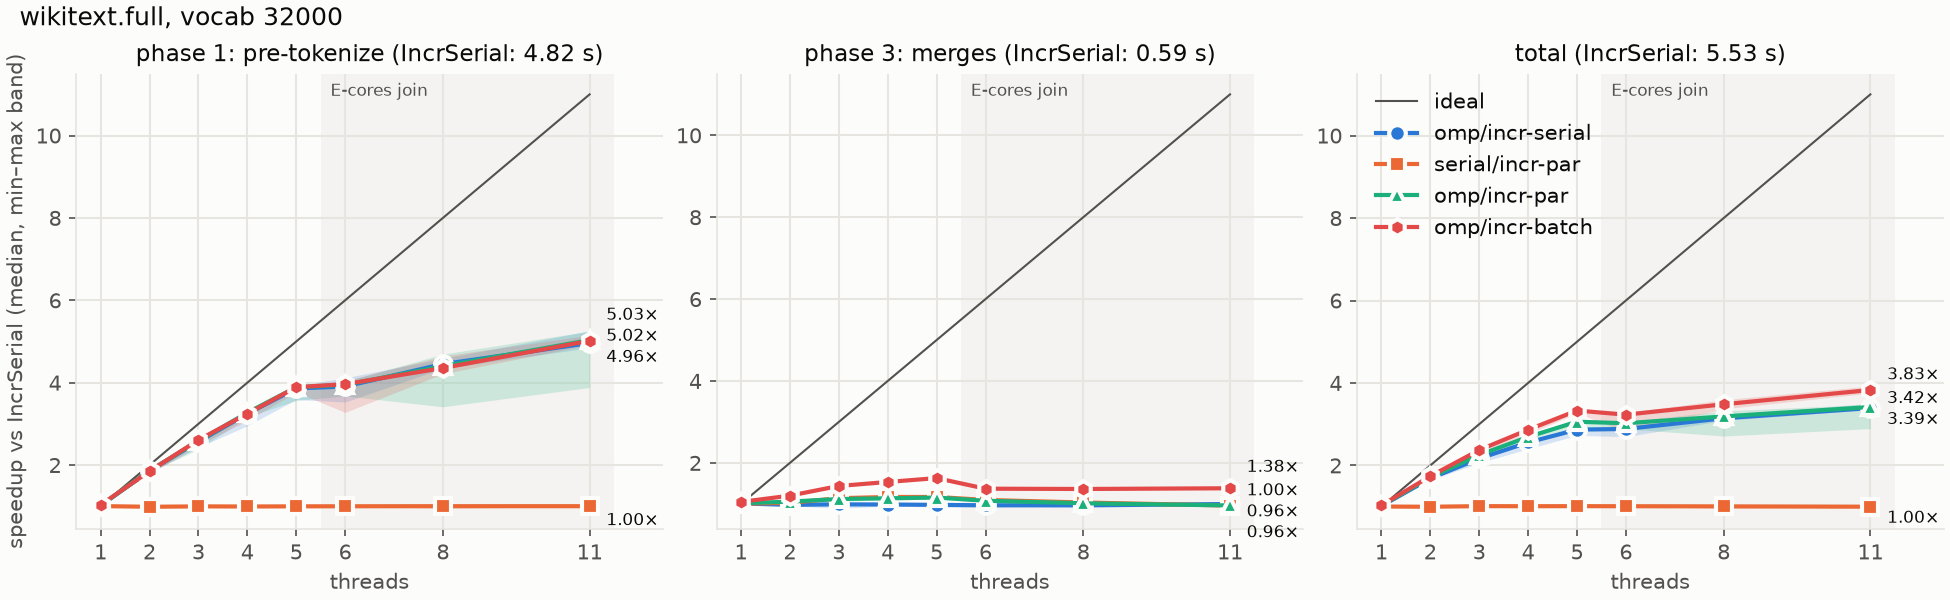
\includegraphics[width=\linewidth]{speedup_wikitext.full_v32000.png}
\caption{WikiText-103, vocabulary 32k: speedup against IncrSerial at 1 thread, per phase (median of 5, band = min--max).
Threads 1--5 run on the performance cores; from 6 the efficiency cores join (shaded).}
\label{fig:speedup}
\end{figure}

With phase 1 parallel, phase 3 dominates what is left. On WikiText-103 IncrSerial's merge phase takes \wtBaseMergeMs\,ms
at vocabulary 32k and \wtBaseMergeMsC\,ms at 100k, and it does not scale at all (\wtSerFive\x{} at 5 threads: it is
serial). Fitting Amdahl's law to the total time on threads 1--5 gives a serial fraction of 0.188 for IncrSerial and
0.132 for \code{incr-batch} (\code{results/plots/summary.md}).

Parallelising inside one merge step does not remove the chain. \code{incr-par} splits each large step across owner
threads and gets \wtParFive\x{} at 5 threads, falling to \wtParEleven\x{} at 11. Below a size threshold a step runs on the
master alone; without that threshold the fork/join cost of 31k parallel regions makes phase 3 \thrZeroFive\,s at
5 threads instead of \thrFourFive\,s (\code{threshold.csv}). The span of the computation is still one step per merge.

\section{Batched rounds and their exactness}

\subsection{The rule}

Sort the live pairs best-first by the specification's order: $q_0 \succ q_1 \succ \dots$ (indices are 0-based).
\begin{enumerate}
\item \textbf{Prefix.} $p[0..K)$ is the longest prefix of that order whose pairs are pairwise token-disjoint, with $K$
  no larger than the remaining merge budget. A self-pair $(a,a)$ may only be the last member.
\item \textbf{Ties.} Let $c^* = \mathrm{count}(p[K{-}1])$ and let $T$ be every live pair ranked after $p[K{-}1]$ with
  count exactly $c^*$, \emph{starting with the entry that stopped the prefix}.
\item \textbf{Keep.} Let $g$ be the number of members with count $> c^*$ and $j$ the first member index whose tokens
  appear in a pair of $T$ ($K$ if none). Merge
  \[ k = \max\bigl(\min(K, j+1),\; g,\; 1\bigr) \]
  members in one round; if the scan of $T$ stopped at its cap, use $k=\max(g,1)$.
\end{enumerate}

\begin{theorem}
From any training state $S$, the next $k$ merges of sequential BPE are exactly $p[0], \dots, p[k{-}1]$, in that order.
\end{theorem}

Write $S_i$ for $S$ after merging $p[0..i)$. The order $\succ$ is strict and total on live pairs: two distinct token ids
with identical bytes would make the specification itself ambiguous, and the vocabulary writer rejects such a run.

\begin{lemma}[old pairs never rise]
Merging $(a,b)\to z$ with $z$ fresh leaves the count of every pair of old tokens at or below its old value, and sets
$\mathrm{count}(a,b)$ to 0.
\end{lemma}

\begin{lemma}[disjoint merges don't interact]
If $\{c,d\}\cap\{a,b\}=\emptyset$, merging $(a,b)$ leaves $\mathrm{count}(c,d)$ unchanged.
\end{lemma}

\begin{lemma}[witness]
Let $i \le K{-}1$ and let $r=(u,v)$ be a pair of $S_i$ with a new token. There is a pair $O$ of old tokens with
$\mathrm{count}_{S_i}(r) \le \mathrm{count}_S(O)$ that shares a token with some $p[l]$, $l<i$, and is not a member.
\end{lemma}

\begin{proof}[Sketch]
New tokens expand to disjoint members, so replace a new token on the left by the second token of its member and one on
the right by the first; every occurrence of $r$ maps to an occurrence of that $O$. If $O$ were a member, disjointness
would force it to be the member it came from, which makes that member a self-pair with index $<K{-}1$, which the prefix
forbids.
\end{proof}

\begin{proof}[Proof of the theorem]
Induction on $i<k$: $p[i]$ is the best pair of $S_i$. By Lemma 2 its count is unchanged. A pair $r$ of old tokens did
not rise (Lemma 1) and ranked after $p[i]$ in $S$, so it still does. A pair $r$ with a new token has a witness $O$ outside
the prefix (Lemma 3), so $\mathrm{count}_S(O)\le c^*$. If $i<g$, $p[i]$ has count $>c^*$ and wins. Otherwise $k>g$ forces
$k=\min(K,j+1)$, so $i\le j$; the members before $i$ share no token with $T$, so $O\notin T$ and
$\mathrm{count}_S(O) < c^* = \mathrm{count}(p[i])$. Either way $p[i]$ beats $r$. With a capped scan $k=\max(g,1)$, and
only the first case arises.
\end{proof}

The comparison with $c^*$ must be strict: on a tie a new pair $(x,z)$ beats its witness $(x,a)$, because the bytes of $z$
extend those of $a$. The index is easy to get wrong. With the words \code{eax}$\times$2 and \code{df}$\times$2 every pair has
count 2 and the order is $(e,a) \succ (d,f) \succ (a,x)$; the prefix is $\{(e,a),(d,f)\}$, $T=\{(a,x)\}$ shares
\code{a} with $p[0]$, so $j=0$ and $k=1$. Sequential BPE indeed merges $(ea,x)$ second, not $(d,f)$. Keeping one member
too many (a 1-based $j$ with $j+1$) is caught by this test and by the runtime oracle.

Members are disjoint, so a round is applied in \emph{one} left-to-right pass per word, with one whole-word difference of
pair counts; a self-pair, always last, is resolved left to right exactly as the greedy rule does.

\section{Implementation}

\paragraph{Selection on the lazy heap.} The master pops live entries (dropping stale ones and adjacent duplicates), builds
the prefix, scans the tie group up to a cap of 4096 entries, and pushes back everything it popped but did not keep
\emph{before} applying the round. The bytes of the new tokens are appended before any heap push, because the heap order
reads them. We kept the lazy max-heap rather than an ordered set: order updates run serially on the master, so they are
part of the Amdahl term.

\paragraph{Hashed owners.} Words are assigned to owners by $\mathrm{mix64}(w \gg 4) \bmod n$ rather than in contiguous
ranges. Words are sorted by their bytes, so a contiguous owner holds all words that share a prefix, and the words of one
pair cluster. Measured on the real engine over every step of at least 4096 tokens, the busiest owner did
\loadContFive\x{} the mean work at 5 threads with contiguous owners and \loadHashFive\x{} with hashed ones
(\loadContEleven\x{} and \loadHashEleven\x{} at 11; Figure~\ref{fig:owners}). One owner per thread was fastest in a sweep of
1, 2 and 4 (\code{b4\_sweep.csv}).

\paragraph{Parallel rounds.} A round whose members touch at least 4096 tokens runs as one OpenMP region: owners rewrite
their words and buffer pair-count changes per thread, pre-bucketed by counts shard; then each shard sums the changes over
threads, so a count never passes through a transient zero or negative value. Pairs that reach zero stay in the owners'
indexes and are erased by a periodic parallel sweep; Lemma 1 guarantees that a zero count stays zero. Rounds too small to
go parallel are cut to a single merge, because one merge is always exact and selection has a cost. This keeps the speed
but raises the round count: \wtDefaultRounds{} rounds at vocabulary 32k against \wtRounds{} when every round is batched.
Span figures in this report come from the latter mode; speedups from the former.

\paragraph{Per-thread state.} Every per-thread buffer written in a hot loop is aligned to 64 bytes.

\section{Verification}

\begin{itemize}
\item \textbf{Golden files.} Eleven small corpora with \code{merges.txt} and \code{vocab.json} from an independent Python
  reference trainer (ties, Unicode 16 classes, emoji, special-token edge cases).
\item \textbf{Equivalence matrix.} Every pre-tokenizer $\times$ engine (plus hashed IncrPar) at threads
  $\{1,2,3,4,8,16\}$ on 10\,MB slices of both corpora must hash identically to the naive serial oracle. Zero mismatches
  after every task.
\item \textbf{Runtime oracle.} \code{-{}-verify-batches} runs a sequential engine alongside and checks each member of each
  round. It passes on WikiText-103 at vocabulary 32k and 100k at 5 and 11 threads. In the unit tests it checks all three
  rules of increasing reach on 200 random corpora, and the parallel engine on 60 more at threads 2, 3, 8 and 16.
\item \textbf{Independent replay.} \code{tools/batchsim} shares no code with the engine, re-derives the batches with an
  ordered set and asserts every member against the sequential argmax; its round counts match the engine's.
\item \textbf{Mutation checks.} Every change to exactness logic was broken on purpose (always $k=K$; a 1-based $j$; $\le$ in
  $g$; the stopping pair left out of $T$; bytes pushed after the heap push; and more): 16 of 17 mutants were caught, the
  survivor being equivalent (it only saves a rescan).
\item \textbf{Races.} ThreadSanitizer runs in CI (Linux), with OpenMP's runtime excluded through Archer's
  \code{ignore\_noninstrumented\_modules}; it is green on every push. ThreadSanitizer and AddressSanitizer do not run
  on this Mac (UBSan does).
\item \textbf{Interoperability.} Our files load into Hugging Face \code{tokenizers}, which encodes held-out text to the
  same ids as the Python reference encoder.
\end{itemize}

Every benchmark row records the sha256 of its \code{merges.txt}. Across all 2{,}232 rows of the final benchmarks, each
input and vocabulary has exactly one hash.

\section{Results}

\paragraph{Setup.} Apple M3 Pro (5 performance + 6 efficiency cores), macOS 27.0.1, Apple clang 17, libomp 22.1.3,
PCRE2 10.45. All timings on mains power; each configuration has a warm-up run and 5 measured repetitions (3 for the
largest inputs), and we report the median. A run whose wall time exceeds twice its CPU time plus 0.05\,s is treated as a
stall (the machine idle-slept during early battery runs) and repeated; none of the final rows stalled. macOS offers no
thread pinning, so threads 1--5 are reported separately from 6--11, where efficiency cores join.

\subsection{Phase 3 speedup}

\begin{table}[h]
\centering\small
\begin{tabular}{llrrrr}
\toprule
 & IncrSerial & \code{incr-par} & \multicolumn{3}{c}{\code{incr-batch}}\\
corpus, vocab & 1 thread & 5 threads & 3 threads & 5 threads & 11 threads\\
\midrule
WikiText-103, 32k & \wtBaseMerge\,s & \wtParFive\x & \wtBatchThree\x & \textbf{\wtBatchFive\x} & \wtBatchEleven\x \\
WikiText-103, 100k & \wtBaseMergeC\,s & \wtParFiveC\x & \wtBatchThreeC\x & \textbf{\wtBatchFiveC\x} & \wtBatchElevenC\x \\
TinyStories 1\,GB, 32k & \tsBaseMerge\,s & \tsParFive\x & \tsBatchThree\x & \tsBatchFive\x & \tsBatchEleven\x \\
\bottomrule
\end{tabular}
\caption{Merge-phase speedup against IncrSerial at 1 thread (\code{batch.csv}, median of 5).}
\label{tab:phase3}
\end{table}

On WikiText-103, batching turns a merge phase that one-merge-per-step parallelism barely moves into a
\wtBatchFive\x{} speedup at 5 threads (Table~\ref{tab:phase3}). The gain shrinks at vocabulary 100k, where later merges
have small counts and many ties, so batches are smaller (span \wtSpanC\x{} against \wtSpan\x). Beyond 5 threads the
efficiency cores slow every round down to their pace, and the speedup drops. The B4 sweep that chose the defaults
measured \killSweep\x{} and \killSweepC\x{} with its own IncrSerial runs (\code{b4\_sweep.csv}), where IncrSerial happened to run slower; the gap is
comparable to the run-to-run spread seen there (up to 12\% min--max for IncrSerial, 22\% for \code{incr-batch}).

On TinyStories the merge phase takes only \tsBaseMergeMs\,ms and batches stay small (Section~\ref{sec:limits}), so no
engine gains: \code{incr-batch} is slightly slower than IncrSerial at 3--5 threads (\tsBatchFive\x) and clearly
slower at 11 (\tsBatchEleven\x).

\paragraph{Whole run.} Pre-tokenizing dominates the total. Against IncrSerial at 1 thread, the full pipeline with
\code{incr-batch} is \wtTotFive\x{} faster at 5 threads and \wtTotEleven\x{} at 11 on WikiText-103 (IncrSerial with the
parallel pre-tokenizer: \wtTotSerFive\x{} and \wtTotSerEleven\x), and \tsTotFive\x{} and \tsTotEleven\x{} on TinyStories.

\subsection{Span and load balance}

\begin{figure}[t]
\centering
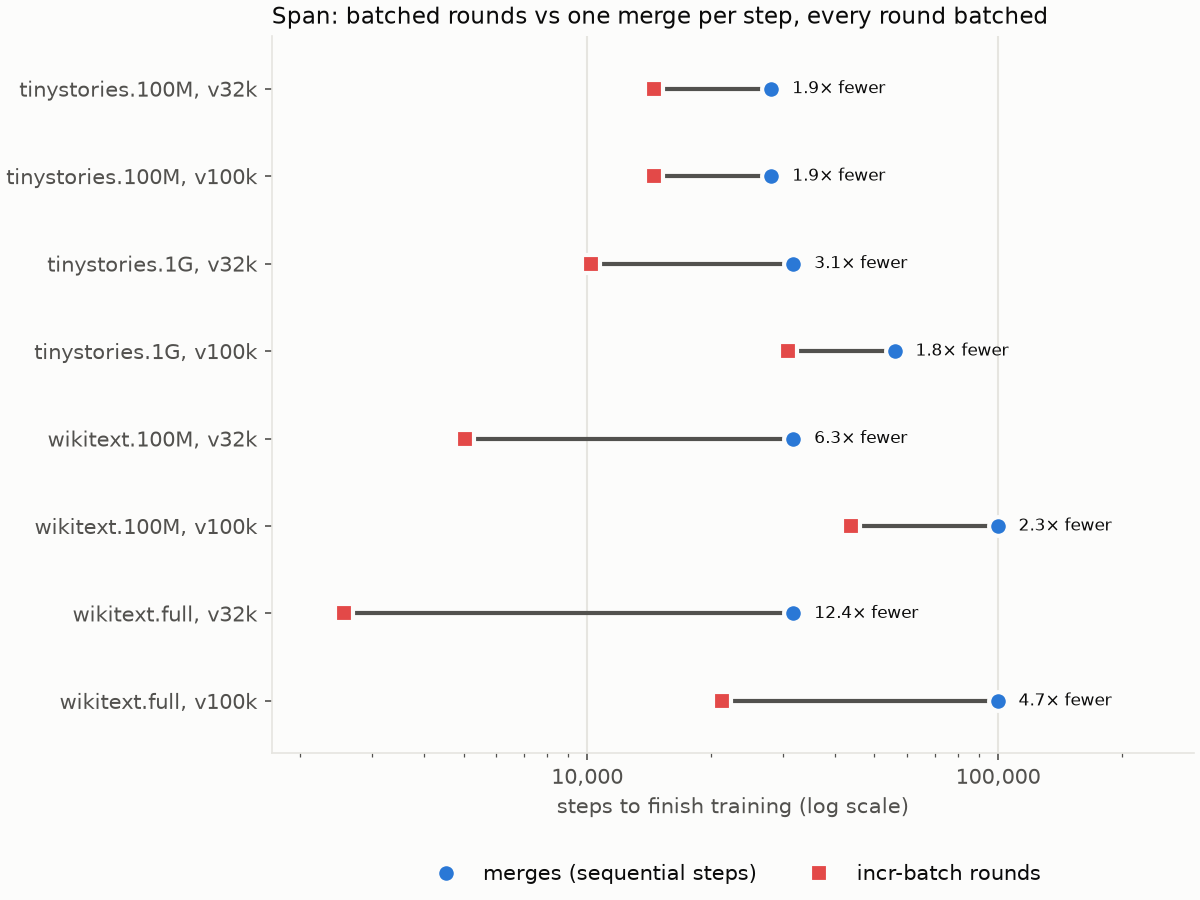
\includegraphics[width=0.62\linewidth]{span.png}
\caption{Sequential steps needed: one per merge (circles) against batched rounds with every round batched (squares).}
\label{fig:span}
\end{figure}

With every round batched, WikiText-103 needs \wtRounds{} rounds for \wtMerges{} merges at 32k (\wtSpan\x{} fewer
sequential steps, up to \wtMaxBatch{} merges in one round) and \wtRoundsC{} rounds for \wtMergesC{} merges at 100k
(\wtSpanC\x). TinyStories gains \tsSpan\x{} (Figure~\ref{fig:span}).

\begin{figure}[t]
\centering
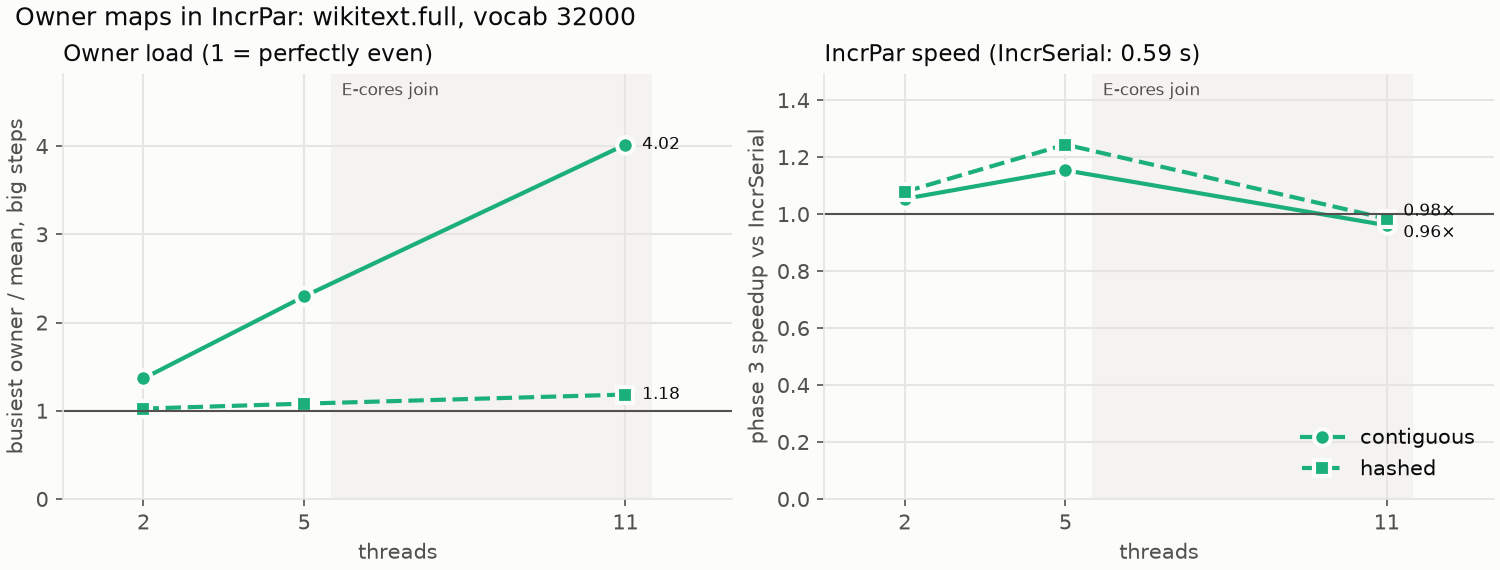
\includegraphics[width=\linewidth]{owners_wikitext.full_v32000.png}
\caption{IncrPar with contiguous and hashed owners, WikiText-103, 32k. Left: busiest owner's tokens over the mean, on
steps of at least 4096 tokens. Right: the effect on IncrPar's merge phase.}
\label{fig:owners}
\end{figure}

Hashing fixes the imbalance but, on its own, barely helps IncrPar: \ownContFive\x{} to \ownHashFive\x{} at 5 threads
(Figure~\ref{fig:owners}). One merge per step leaves too little work per parallel region. The gain of \code{incr-batch} comes
from the batched rounds, with hashed owners keeping each round balanced.

\subsection{What the trace shows}

\code{-{}-trace} records per-thread events (selection, owner rewrites, reductions, order updates) into 64-byte-aligned
buffers; with tracing off the run is unchanged within noise, and tracing on costs \ohOn\% and \ohOnC\% of the merge phase
at 32k and 100k (\code{trace\_overhead.md}). At 5 threads on WikiText-103 (32k), the master is busy for \traceMaster\,ms of
the merge phase and each worker for about \traceWorker\,ms: the serial selection and order updates on the master now bound
the speedup. A selection takes \traceSelectMean\,$\mu$s on average. The trace also samples the CPU each event started on: in an
11-thread run, six of the ten workers were on efficiency cores for all of their merge-phase work and the master for none
of it (\code{trace\_wikitext.full\_v32000\_t11.md}), so every parallel round waits for an efficiency core.

\subsection{Scale points}

\begin{table}[h]
\centering\small
\begin{tabular}{lrrrr}
\toprule
 & serial & \multicolumn{2}{c}{\code{incr-batch}, 11 threads} & phase 3,\\
input & total & total & speedup & 5 threads\\
\midrule
TinyStories full (\scTsGB\,GB), 32k & \scTsSerial\,s & \scTsBatchEleven\,s & \scTsTotEleven\x & \scTsBatchFive\x\\
TinyStories full, 100k & \scTsSerialC\,s & \scTsBatchElevenC\,s & \scTsTotElevenC\x & \scTsBatchFiveC\x\\
WikiText $\times$6 (\scWxGB\,GB), 32k & \scWxSerial\,s & \scWxBatchEleven\,s & \scWxTotEleven\x & \scWxBatchFive\x\\
WikiText $\times$6, 100k & \scWxSerialC\,s & \scWxBatchElevenC\,s & \scWxTotElevenC\x & \scWxBatchFiveC\x\\
\bottomrule
\end{tabular}
\caption{Largest inputs (\code{scale.csv}, median of 3). WikiText $\times$6 is six copies of WikiText-103: more bytes, the
same unique words, so its merge phase equals WikiText-103's.}
\end{table}

\subsection{Comparison with Hugging Face \code{tokenizers}}

On the 100\,MB WikiText slice at 32k, Hugging Face \code{tokenizers} 0.23.3 takes \wtHFOne\,s with one thread and
\wtHFEleven\,s with 11; ParaBPE takes \wtOursEleven\,s at 11 threads. On TinyStories the figures are \tsHFOne\,s,
\tsHFEleven\,s and \tsOursEleven\,s. These are single runs from a profiling script, not the benchmark protocol, and
HF breaks ties by pair id rather than by our byte order, so its merge list differs slightly on TinyStories
(\tsHFMerges{} merges against our \tsOursMerges, where the corpus runs out of pairs).

\begin{figure}[t]
\centering
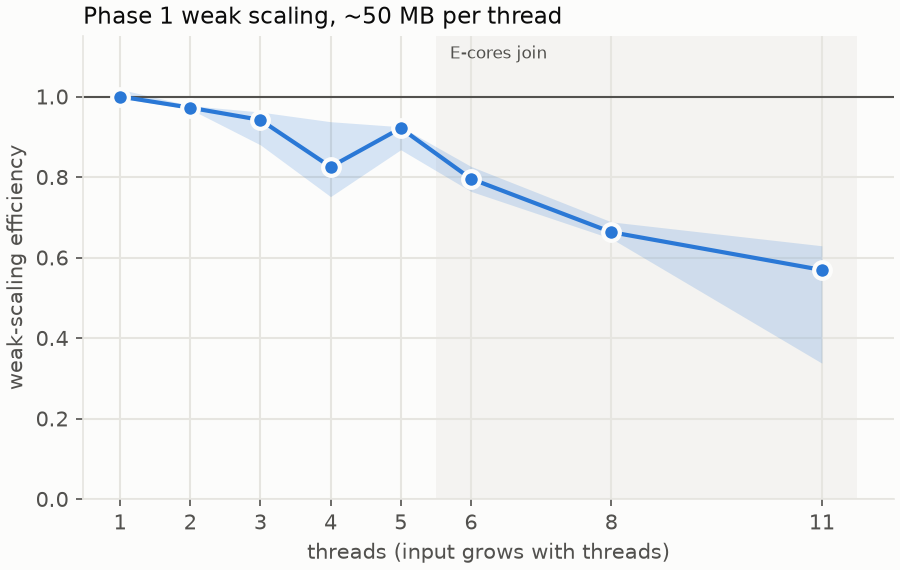
\includegraphics[width=0.6\linewidth]{weak_scaling.png}
\caption{Phase 1 weak scaling on TinyStories slices, about 50\,MB per thread.}
\label{fig:weak}
\end{figure}

\section{Limits}
\label{sec:limits}

\begin{itemize}
\item \textbf{Tie-heavy corpora.} On TinyStories most rounds are single merges (\tsDefaultRounds{} rounds for \tsMerges{}
  merges at 32k): the vocabulary is small and repetitive, ties are frequent, and the merge phase is a few tens of
  milliseconds, so the batching machinery has nothing to amortise.
\item \textbf{The master is serial.} Selection and order updates are the remaining Amdahl term (Section 8.3).
\item \textbf{One machine, no pinning.} All results come from one laptop. macOS cannot pin threads, so the scheduler places
  them; the P/E labels in traces are samples, not placements.
\item \textbf{Power.} Early runs on battery were slowed by idle sleep; every result reported here was rerun on mains power,
  and stalled runs are detected and repeated.
\item \textbf{Sanitizers are CI-only.} ThreadSanitizer and AddressSanitizer run on Linux in CI; the local ASan build hangs
  on this Mac.
\item \textbf{The proof assumes} a strict total order on pairs, which needs distinct bytes for distinct tokens; a
  violating run fails loudly rather than producing a wrong file.
\end{itemize}

\section{Related work}

Batching BPE merges is not new: BatchBPE (Morgan, 2024) merges many pairs per batch, but it runs them serially, changes
the merge order, and argues informally that the vocabulary differs at most in a ``tiny difference'' near the end of
training (its \S3.6). Parallel BPE training is not new either: Hugging Face \code{tokenizers} and YouTokenToMe parallelise
the words of one merge, as our \code{incr-par} does. Zouhar et al.\ (2023) characterise when merge sequences are
equivalent, and our rounds have the shape of Blelloch et al.'s deterministic reservations, with the difference that the BPE
task list is not known in advance. Two-phase BoundlessBPE (2026) is single-threaded and applies one merge per iteration.

As of our search (November 2026), we found no prior BPE trainer that applies several merges per parallel round with a proof
that the merge list, including order and tie-breaking, is byte-identical to sequential training. A search cannot show that
something doesn't exist; sources and limits are in \code{docs/notes/related\_work.md}.

\section{Conclusion}

The merge chain of BPE training looks inherently sequential, but much of it is not: on WikiText-103 a closed-form rule
finds batches that cover \wtSpan\x{} fewer steps, and a proof shows they reproduce sequential training byte for byte. On a
laptop with 5 performance cores this turns the merge phase from \wtParFive\x{} into \wtBatchFive\x{}, with every output
checked against the serial baseline. The next limit is the serial master: parallel selection is the obvious next step.

\appendix
\section{Reproducing}
\begin{verbatim}
cmake -B build -DCMAKE_BUILD_TYPE=Release && cmake --build build -j
ctest --test-dir build --output-on-failure
.venv/bin/python -I bench/run_bench.py bench/configs/batch.yaml --require-ac
.venv/bin/python -I bench/plot.py results/*.csv --out-dir results/plots
.venv/bin/python -I report/numbers.py        # regenerates report/numbers.tex
\end{verbatim}

\end{document}
